\chapter{Ajuan Sistem Baru}

\section{Rancangan Sistem Baru}

\subsection{Rancangan Latihan Klasifikasi}

Rancangan sistem untuk tahap latihan klasifikasi disajikan dalam bagan pada Gambar \ref{fig:design_training} berikut. Proses-proses yang harus dilewati dalam tahap latihan klasifikasi dapat dijelaskan sebagai berikut:

\begin{enumerate}
	\item sistem akan memuat \textit{file} JSON yang berisi data latihan yang digunakan untuk membangun NLU,
	\item sistem mengambil data latihan tersebut lalu mengubahnya menjadi sekumpulan obyek SentenceData,
	\item sistem mengambil informasi maksud kalimat yang telah didefinisikan di dalam data latihan dan menyimpan sekumpulan maksud kalimat,
	\item sistem memecahkan sebuah kalimat menjadi sekumpulan \textit{token} kata,
	\item sistem mengekstraksi entitas yang telah didefinisikan di dalam data latihan dan mengumpulkan semua entitas yang terekstrasi,
	\item sistem menciptakan tas kata-kata dengan menggunakan metode \textit{one-hot encoding},
	\item sekumpulan maksud kalimat dan tas kata-kata digunakan sebagai masukan untuk latihan model NLU, menghasilkan model klasifikasi, dan,
	\item model klasifikasi disimpan ke dalam direktori sistem untuk digunakan pada tahap klasifikasi teks.
\end{enumerate}

\begin{figure}[H]
	\centering
	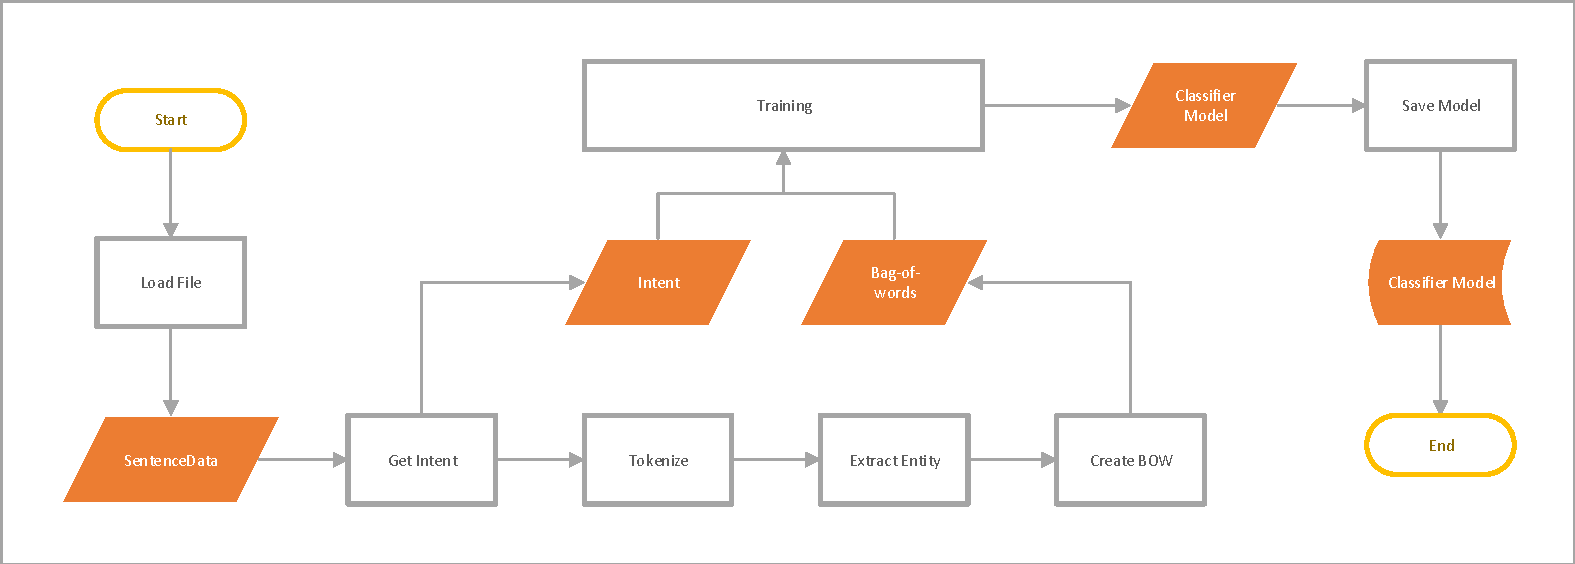
\includegraphics[width=\textwidth, trim=2 2 2 2, clip]{resources/4-design_training.pdf}
	\caption{Bagan rancangan sistem tahap latihan klasifikasi}
	\label{fig:design_training}
\end{figure}

\subsection{Rancangan Klasifikasi Teks}

Rancangan sistem untuk tahap klasifikasi teks disajikan dalam bagan pada Gambar \ref{fig:design_classification}. Proses-proses yang harus dilewati dalam tahap klasifikasi teks dapat dijelaskan sebagai berikut:

\begin{enumerate}
	\item sistem menerima masukan teks dari \textit{speech recognition} yang dimasukkan oleh suara pengguna,
	\item sistem memecahkan teks menjadi sekumpulan \textit{token},
	\item sistem mengenali entitas yang berada di dalam teks, kemudian mengekstraksi entitas tersebut,
	\item sistem menciptakan tas kata-kata untuk teks masukan,
	\item sistem melakukan prediksi maksud kalimat dari masukan tas kata-kata menggunakan model klasifikasi yang dihasilkan pada tahap latihan klasifikasi,
	\item maksud kalimat yang telah dihasilkan, bersama dengan kumpulan entitas hasil ekstrasi, menjadi masukan untuk memenggil aksi sistem, dan,
	\item sistem melakukan aksi kepada pengguna sebagai tanggapan dari masukan teks dari sistem ASR.
\end{enumerate}

\begin{figure}[H]
	\centering
	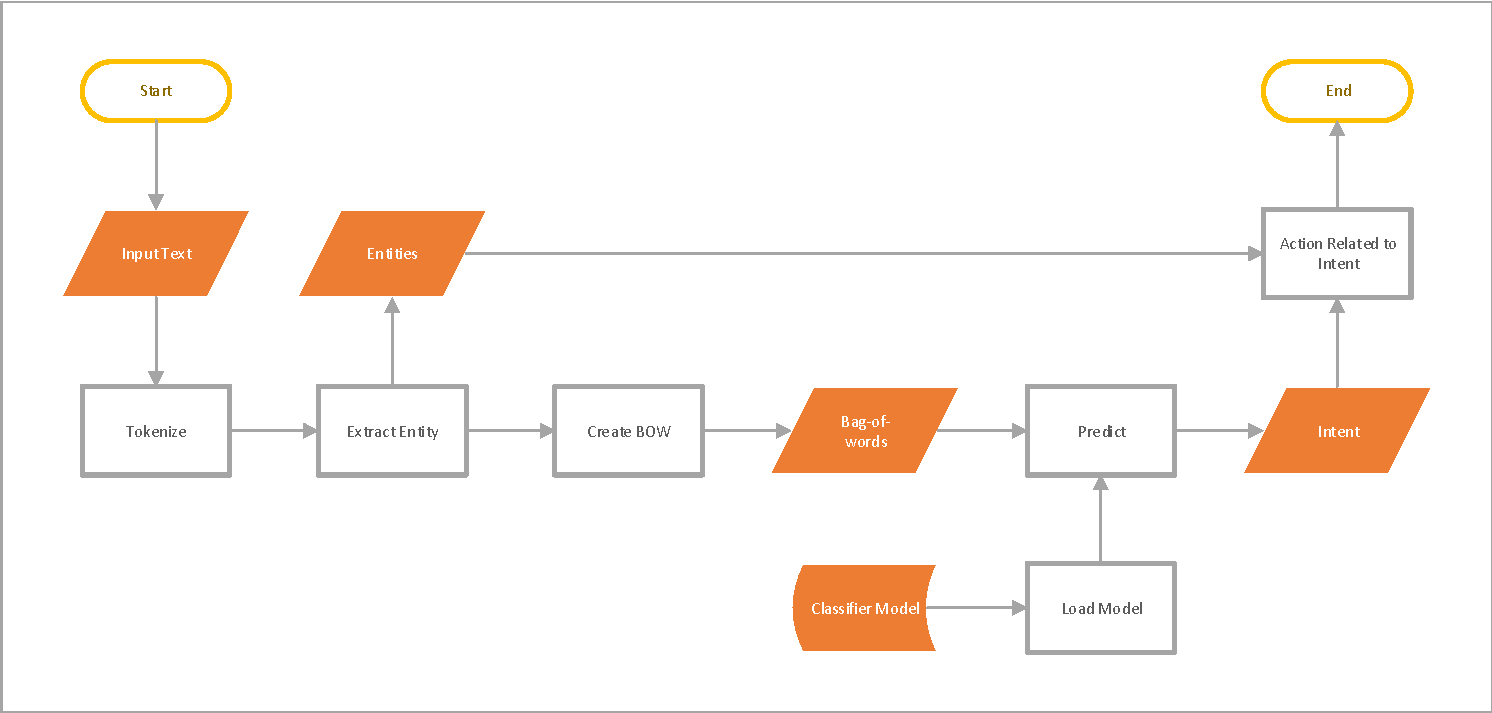
\includegraphics[width=\textwidth, trim=2 2 2 2, clip]{resources/4-design_classification.pdf}
	\caption{Bagan rancangan sistem tahap klasifikasi teks}
	\label{fig:design_classification}
\end{figure}

\section{Penjelasan Proses}

\subsection{Memuat Data}

Data latihan yang disediakan di dalam direktori sistem memiliki format JSON. Data tersebut berisikan teks yang akan dilatih beserta informasi maksud kalimat dan entitas yang terkandung di dalamnya jika ada. Dalam tahap latihan klasifikasi, sistem akan memuat data latihan dan memasukkan data-data menjadi obyek SentenceData. Obyek SentenceData memiliki atribut-atribut berupa teks, \textit{token-token}, dan tanda entitas tiap \textit{token}. Selain itu, proses memuat data juga menghasilkan nilai entitas yang terkandung di dalam kalimat data latihan.

\subsection{Tokenisasi}

Tokenisasi adalah proses untuk memecahkan sebuah teks kalimat menjadi sekumpulan \textit{token}. Selain kata dan angka, \textit{token} dapat juga berbentuk tanda baca. Rancangan proses tokenisasi untuk sistem NLU baru yang akan dibangun ditunjukkan dalam bagan pada Gambar \ref{fig:design_token}. Teks yang dihadapi oleh sistem berupa kalimat yang dibentuk dari huruf-huruf tanpa tanda baca, mengingat bahwa teks merupakan keluaran dari sistem ASR. Teks dipecahkan dengan menggunakan prosedur split() yang telah disediakan oleh Python. Hasil pecahan teks disimpan kembali ke dalam obyek SentenceData.

\begin{figure}[H]
	\centering
	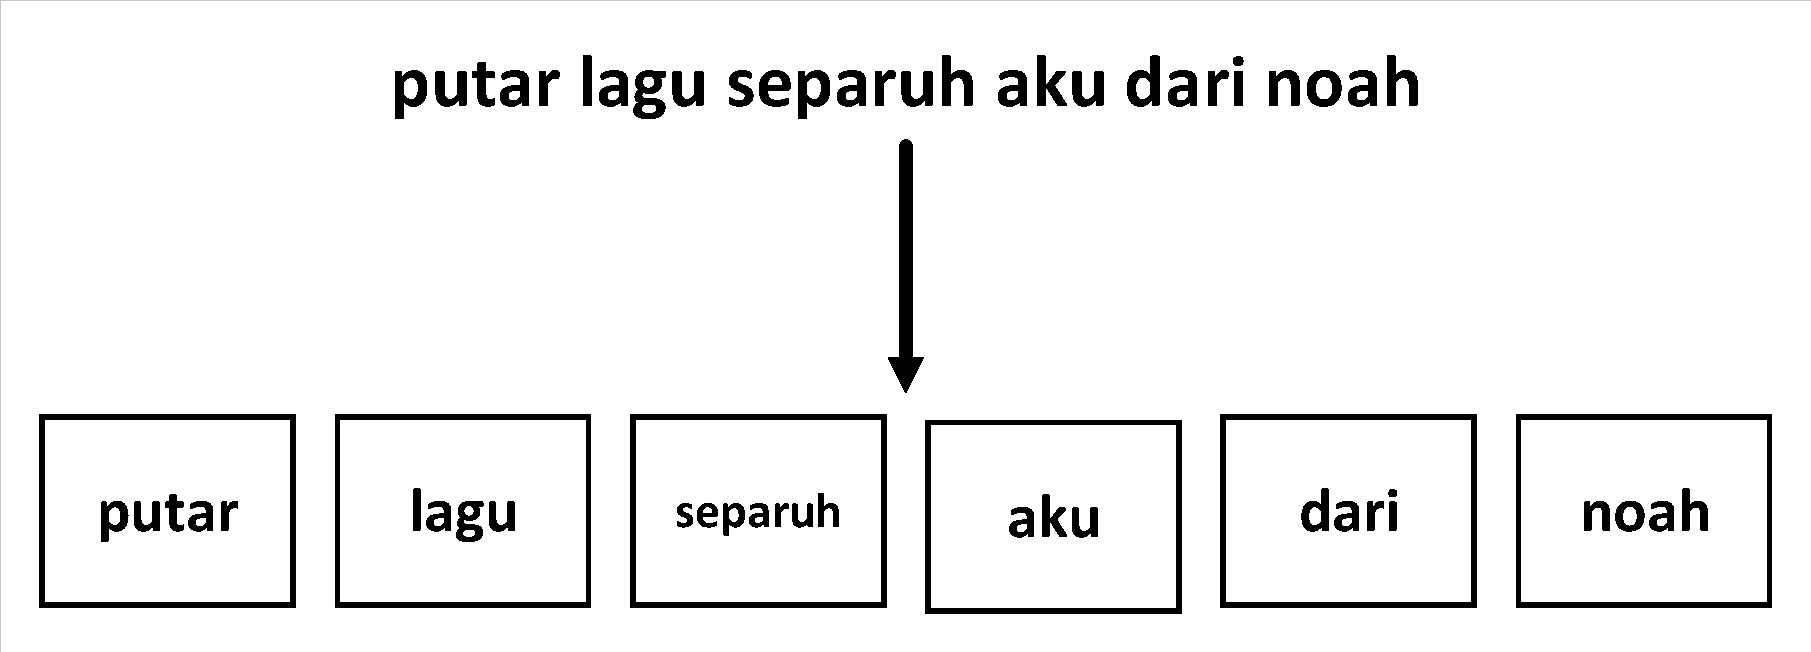
\includegraphics[width=0.8\textwidth, trim=2 2 2 2, clip]{resources/4-design_token.pdf}
	\caption{Rancangan proses tokenisasi}
	\label{fig:design_token}
\end{figure}

\subsection{Ekstraksi Entitas}

Ekstraksi entitas adalah proses untuk mengambil entitas-entitas yang terkandung di dalam teks. Entitas tersebut akan digunakan sebagai masukan aksi yang akan dijalankan sistem NLU setelah memprediksi maksud kalimat dari teks tersebut.

Gambar \ref{fig:design_entity} menunjukkan rancangan untuk proses ekstraksi entitas dalam sistem NLU baru. Dalam tahap latihan klasifikasi, entitas-entitas yang ada di dalam teks telah didefinisikan di dalam data latihan. Sistem akan menandakan token mana saja yang termasuk ke dalam entitas tersebut dengan menggunakan skema BILUO [cit]. Penanda tersebut akan berguna untuk melakukan latihan pengenalan entitas, yang mana model hasil dari latihan tersebut disimpan ke dalam direktori sistem. Untuk proses latihan klasifikasi, semua \textit{token} yang merupakan entitas diganti menjadi satu \textit{token} yang bernilai nama entitas tersebut.

Dalam tahap klasifikasi teks, sebuah teks polos masukan dari sistem ASR akan ditebak entitas-entitas di dalamnya dengan menggunakan model latihan pengenalan entitas yang telah dijalankan sebelumnya. Setelah semua token telah ditandai, sistem akan mengambil nilai entitas-entitas yang terkandung dan menyimpan nilai tersebut untuk digunakan setelah klasifikasi maksud teks telah dijalankan.

\begin{figure}[H]
	\centering
	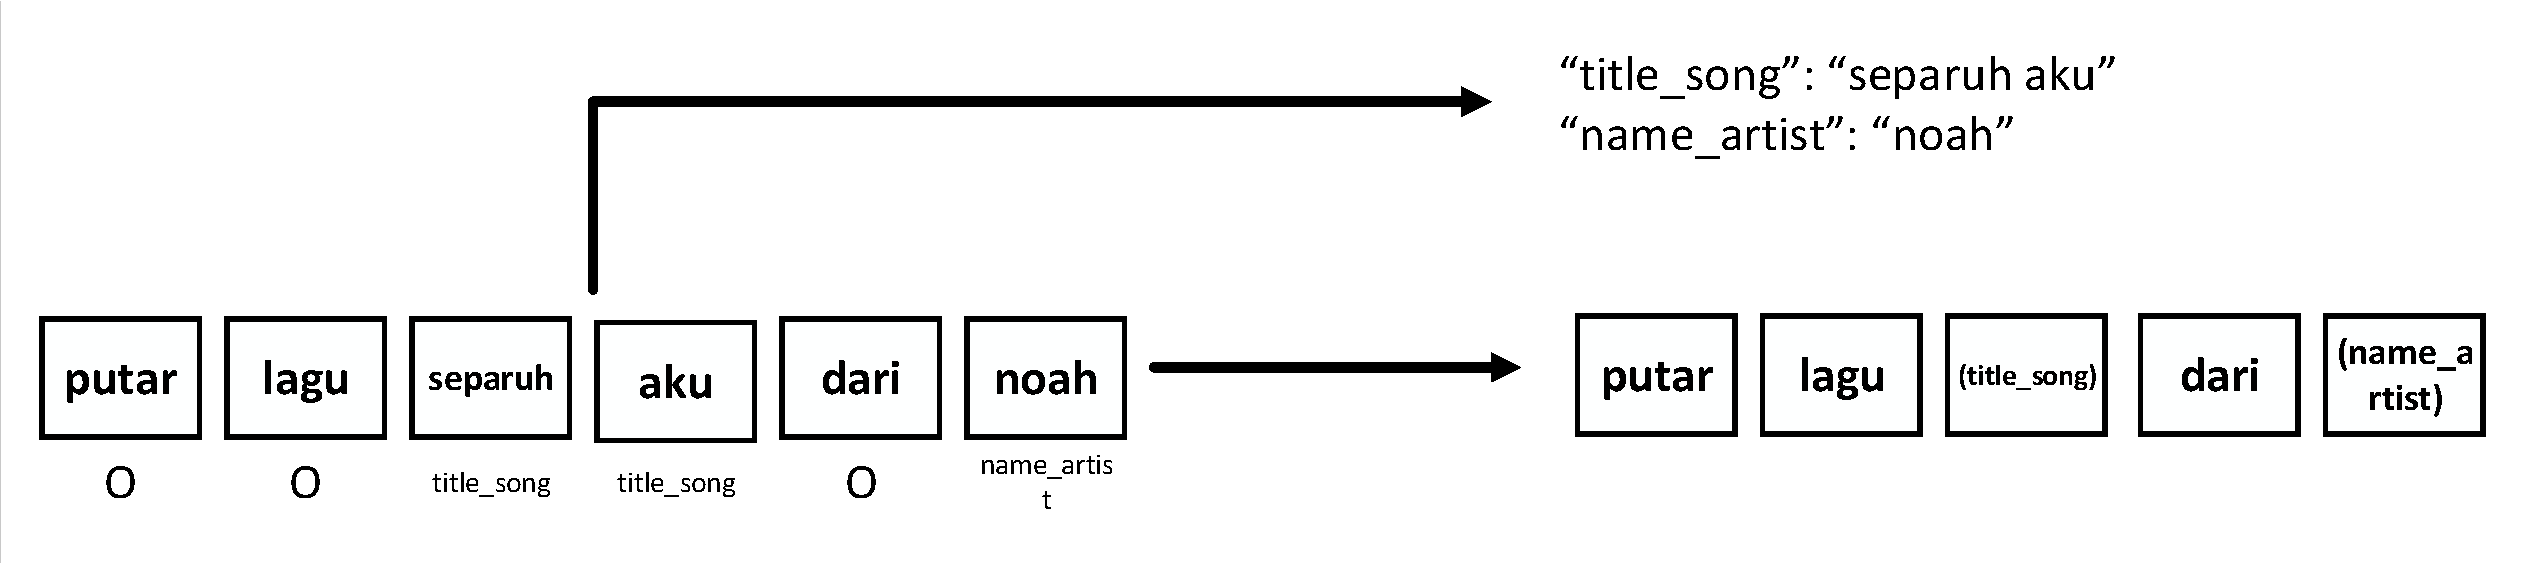
\includegraphics[width=\textwidth, trim=2 2 2 2, clip]{resources/4-design_entity.pdf}
	\caption{Rancangan proses ekstraksi entitas}
	\label{fig:design_entity}
\end{figure}

Rasa NLU memiliki beberapa jenis pilihan metode untuk melakukan latihan pada proses ini. Namun, pilihan yang cocok dengan permasalahan ini adalah latihan pengenalan entitas dengan menggunakan conditional random field (CRF). Hal ini dikarenakan metode CRF adalah salah satu dari dua metode yang mendukung nama entitas selain nama standar entitas.

Penggunaan CRF dalam mengenali entitas dapat diperbaiki dengan menggunakan algoritma-algoritma yang lain. Beberapa pilihan algoritma yang cocok adalah sebagai berikut:

\begin{enumerate}
	\item menggunakan \textit{recurrent neural network} dari Keras,
	\item menggunakan \textit{convolutional neural network} dari Keras,
	\item menggunakan \textit{convolutional neural network} dua arah [cit],
\end{enumerate}

\subsection{Menciptakan Tas Kata-Kata}

Tas kata-kata, atau lebih dikenal dengan \textit{bag-of-words} (BOW), adalah bentuk representasi sebuah kalimat dengan menunjukkan kehadiran kata-kata dalam kosakata di dalam kalimat tersebut. Pembentukan tas kata-kata dapat dilihat pada Gambar \ref{fig:design_bow}. Tas kata-kata diciptakan dengan menggunakan teknik \textit{one-hot encoding}, yaitu merepresentasikan kosakata yang muncul di dalam sebuah kalimat ke dalam bentuk biner. Pembuatan kosakata dilakukan dengan melacak semua kata yang muncul di dalam data latihan yang telah diberikan. Untuk kata-kata yang menjadi entitas, kata tersebut diganti menjadi satu token berisi nama entitas.

\begin{figure}[H]
	\centering
	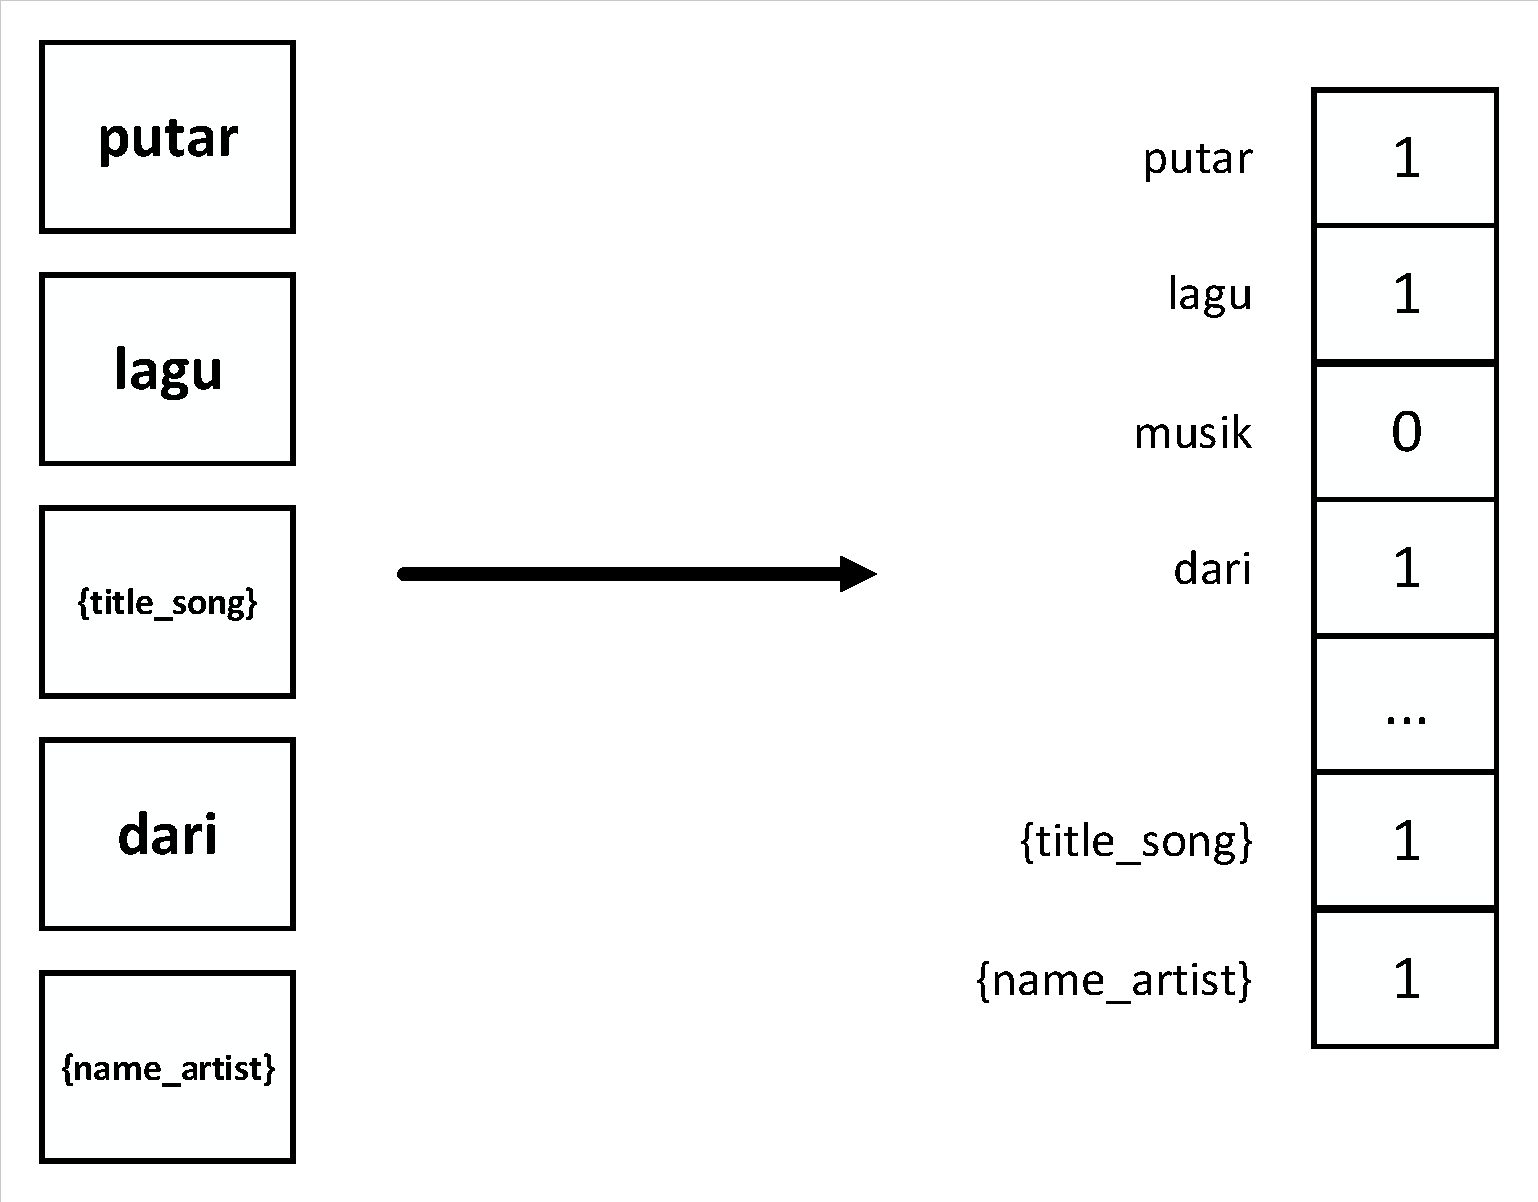
\includegraphics[width=0.5\textwidth, trim=3 3 3 3, clip]{resources/4-design_bow.pdf}
	\caption{Rancangan proses menciptakan tas kata-kata}
	\label{fig:design_bow}
\end{figure}

\subsection{Latihan Klasifikasi}

Latihan dijalankan untuk melatih sekumpulan tas kata-kata dan maksud kalimat yang terlibat, kemudian menciptakan model hasil latihan dan menyimpannya ke dalam direktori sistem. Gambar \ref{fig:design_train_class} menunjukkan bagaimana sistem melakukan latihan dan menciptakan model latihan. Sistem mendapatkan sekumpulan tas kata-kata dan label maksud kalimat secara bersamaan. Tas kata-kata menjadi masukan contoh masukan model, sedangkan label maksud kalimat menjadi masukan contoh keluaran model.

\begin{figure}[H]
	\centering
	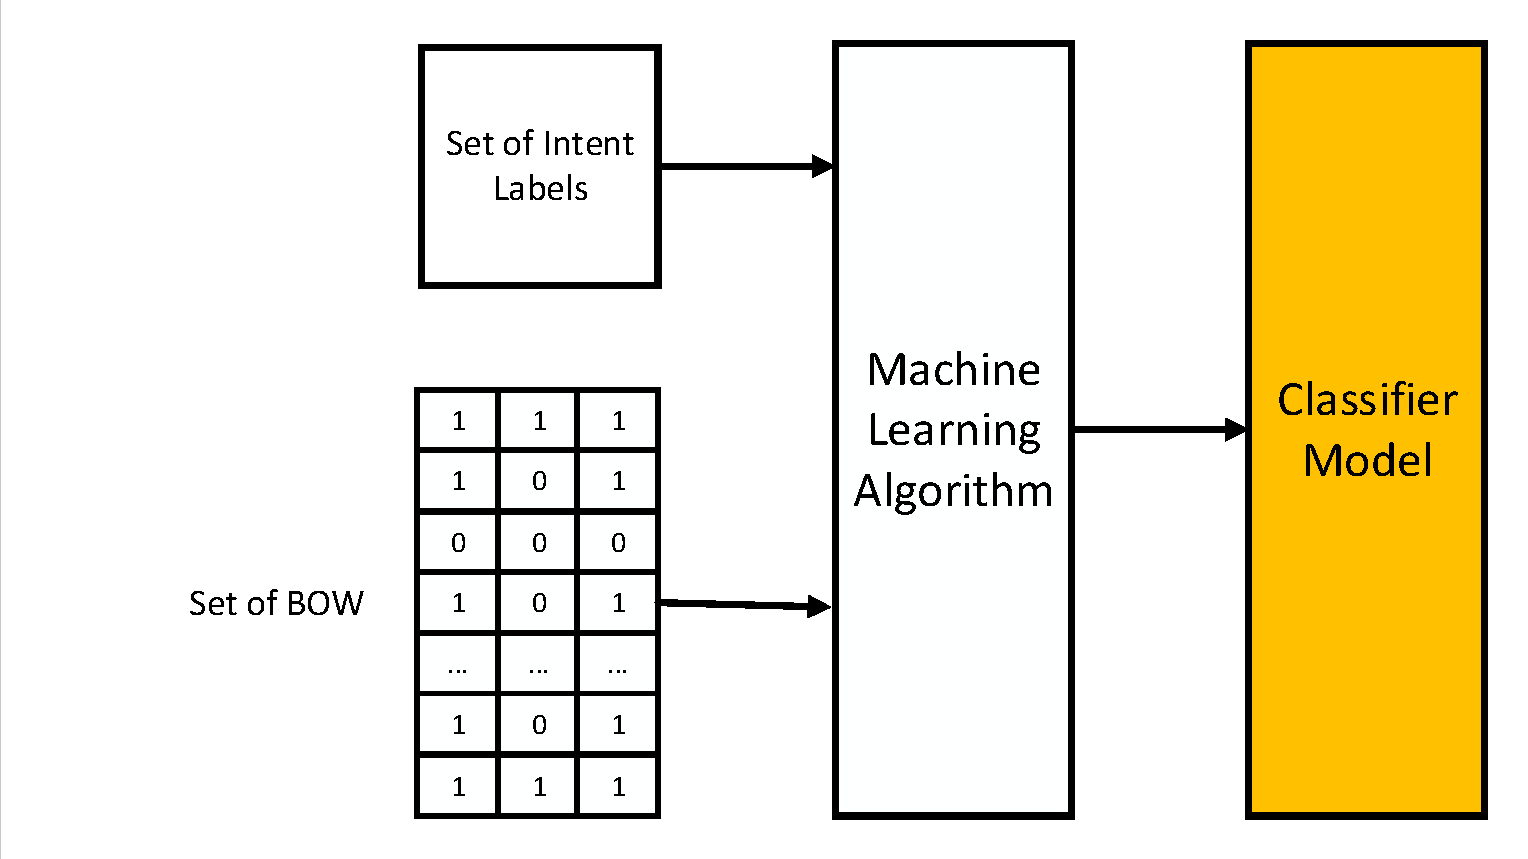
\includegraphics[width=0.7\textwidth, trim=3 3 3 3, clip]{resources/4-design_train_class.pdf}
	\caption{Rancangan proses latihan klasifikasi}
	\label{fig:design_train_class}
\end{figure}

Dalam Rasa NLU, latihan klasifikasi dijalankan dengan menggunakan \textit{support vector machine} (SVM) dengan tambahan \textit{cross-validation} dan optimasi berbasis \textit{grid-search} dari scikit-learn. Untuk sistem NLU yang baru, terdapat beberapa pilihan yang bisa digunakan sebagai latihan klasifikasi, yaitu sebagai berikut:

\begin{enumerate}
	\item menggunakan SVM dengan tambahan \textit{cross-validation} dan optimasi berbasis \textit{random search} dari scikit-learn,
	\item menggunakan \textit{artificial neural network} dari Keras,
\end{enumerate}

\subsection{Klasifikasi}

Proses klasifikasi dijalankan pada tahap klasifikasi teks. Gambaran mengenai proses ini terdapat pada Gambar \ref{fig:design_class_class}. Sistem terlebih dahulu memuat model latihan yang telah disimpan di dalam direktori sistem. Lalu, sistem menggunakan model tersebut untuk melakukan prediksi dari teks masukan yang telah diubah menjadi sebuah tas kata-kata.

\begin{figure}[H]
	\centering
	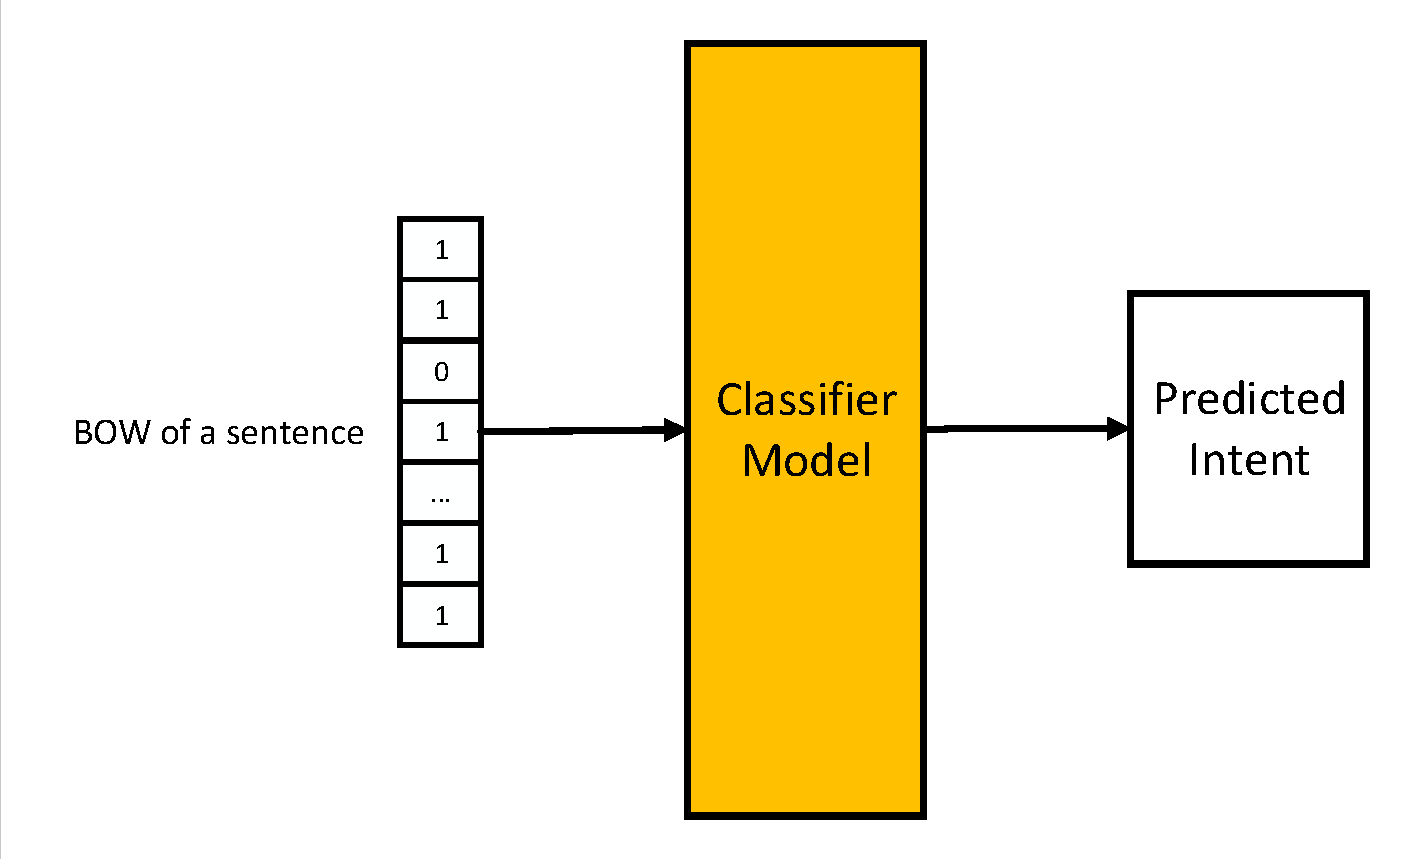
\includegraphics[width=0.7\textwidth, trim=2 2 2 2, clip]{resources/4-design_class_class.pdf}
	\caption{Rancangan proses klasifikasi}
	\label{fig:design_class_class}
\end{figure}

\subsection{Memanggil Aksi Sistem}

Maksud kalimat yang telah diprediksi di tahap klasifikasi teks, digunakan untuk memilih aksi yang akan dilakukan oleh sistem NLU kepada pengguna sistem. Aksi sistem ini pada umumnya adalah melakukan komunikasi REST API kepada sistem API SVARA. API SVARA akan memberikan respon berupa \textit{file} JSON kepada sistem NLU jika komunikasi sukses dijalankan. Kemudian, \textit{file} JSON yang diterima oleh sistem NLU diberikan kepada aplikasi yang dimiliki oleh pengguna secara langsung. Pengolahan \textit{file} JSON setelah berada di aplikasi pengguna diserahkan kepada aplikasi itu sendiri.

Beberapa aksi memerlukan parameter masukan untuk dapat melengkapi komunikasi dengan API SVARA. Parameter masukan didapatkan dari entitas-entitas yang telah diambil nilainya setelah tiap \textit{token} kalimat ditandai pada saat proses ekstraksi entitas.

\section{Perbandingan Hasil Latihan}

\subsection{Latihan Pengenalan Entitas}

\subsection{Latihan Klasifikasi Maksud Kalimat}